%%%%%%%%%%%%%%%%%% INTRODUCTION %%%%%%%%%%%%%%%%%%
\documentclass[border=10pt]{standalone}

%%%%%%%%%%%%%%%%%% PACKAGE %%%%%%%%%%%%%%%%%%
\usepackage{tikz}%  permet de dessiner des figures, des graphiques
\usepackage{adjustbox}% permet de déterminer une taille de fenêtre

%%  FONT
\usepackage[utf8]{inputenc}
\usepackage[T1]{fontenc}

\usepackage{tgadventor}% paquet de police de caractère TGadventor
\usepackage{sansmath}%  Copie-colle la police active dans \sfdefault (/!\ N'EST PAS UNE POLICE DE CARACTÈRES)

%%%%%%%%%%%%%%%%%% SETUP %%%%%%%%%%%%%%%%%%
\tikzset{pictparam/.style={font={\sansmath\sffamily}, thick, line cap=round, line join=round, >=latex, x=1.0cm, y=1.0cm, scale=1}}

%%%%%%%%%%%%%%%%%% DOCUMENT %%%%%%%%%%%%%%%%%%
\begin{document}
\begin{adjustbox}{width={15cm},totalheight={15cm},keepaspectratio}
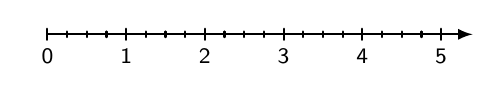
\begin{tikzpicture}[pictparam]
    \draw[->] (0,0) -- (5+0.4,0);
    \foreach \x in {0,0.25,...,5}
	{	\draw[shift={(\x,0)},color=black] (0pt,1pt) -- (0pt,-1pt);
	}
    \foreach \x in {0,...,5}
	{	\draw[shift={(\x,0)},color=black] (0pt,2pt) -- (0pt,-2pt);
		\draw[shift={(\x,0)},color=black] (0,0) node[inner sep=5pt, below] {\footnotesize $\x$};
	}
\end{tikzpicture}
\end{adjustbox}
\end{document}